%% bare_conf.tex
%% V1.4b
%% 2015/08/26
%% by Michael Shell
%% See:
%% http://www.michaelshell.org/
%% for current contact information.
%%
%% This is a skeleton file demonstrating the use of IEEEtran.cls
%% (requires IEEEtran.cls version 1.8b or later) with an IEEE
%% conference paper.
%%
%% Support sites:
%% http://www.michaelshell.org/tex/ieeetran/
%% http://www.ctan.org/pkg/ieeetran
%% and
%% http://www.ieee.org/

%%*************************************************************************
%% Legal Notice:
%% This code is offered as-is without any warranty either expressed or
%% implied; without even the implied warranty of MERCHANTABILITY or
%% FITNESS FOR A PARTICULAR PURPOSE! 
%% User assumes all risk.
%% In no event shall the IEEE or any contributor to this code be liable for
%% any damages or losses, including, but not limited to, incidental,
%% consequential, or any other damages, resulting from the use or misuse
%% of any information contained here.
%%
%% All comments are the opinions of their respective authors and are not
%% necessarily endorsed by the IEEE.
%%
%% This work is distributed under the LaTeX Project Public License (LPPL)
%% ( http://www.latex-project.org/ ) version 1.3, and may be freely used,
%% distributed and modified. A copy of the LPPL, version 1.3, is included
%% in the base LaTeX documentation of all distributions of LaTeX released
%% 2003/12/01 or later.
%% Retain all contribution notices and credits.
%% ** Modified files should be clearly indicated as such, including  **
%% ** renaming them and changing author support contact information. **
%%*************************************************************************


% *** Authors should verify (and, if needed, correct) their LaTeX system  ***
% *** with the testflow diagnostic prior to trusting their LaTeX platform ***
% *** with production work. The IEEE's font choices and paper sizes can   ***
% *** trigger bugs that do not appear when using other class files.       ***                          ***
% The testflow support page is at:
% http://www.michaelshell.org/tex/testflow/



\documentclass[conference]{IEEEtran}
% Some Computer Society conferences also require the compsoc mode option,
% but others use the standard conference format.
%
% If IEEEtran.cls has not been installed into the LaTeX system files,
% manually specify the path to it like:
% \documentclass[conference]{../sty/IEEEtran}





% Some very useful LaTeX packages include:
% (uncomment the ones you want to load)


% *** MISC UTILITY PACKAGES ***
%
% \usepackage{ifpdf}
% Heiko Oberdiek's ifpdf.sty is very useful if you need conditional
% compilation based on whether the output is pdf or dvi.
% usage:
% \ifpdf
%   % pdf code
% \else
%   % dvi code
% \fi
% The latest version of ifpdf.sty can be obtained from:
% http://www.ctan.org/pkg/ifpdf
% Also, note that IEEEtran.cls V1.7 and later provides a builtin
% \ifCLASSINFOpdf conditional that works the same way.
% When switching from latex to pdflatex and vice-versa, the compiler may
% have to be run twice to clear warning/error messages.






% *** CITATION PACKAGES ***
%
\usepackage{cite}
% cite.sty was written by Donald Arseneau
% V1.6 and later of IEEEtran pre-defines the format of the cite.sty package
% \cite{} output to follow that of the IEEE. Loading the cite package will
% result in citation numbers being automatically sorted and properly
% "compressed/ranged". e.g., [1], [9], [2], [7], [5], [6] without using
% cite.sty will become [1], [2], [5]--[7], [9] using cite.sty. cite.sty's
% \cite will automatically add leading space, if needed. Use cite.sty's
% noadjust option (cite.sty V3.8 and later) if you want to turn this off
% such as if a citation ever needs to be enclosed in parenthesis.
% cite.sty is already installed on most LaTeX systems. Be sure and use
% version 5.0 (2009-03-20) and later if using hyperref.sty.
% The latest version can be obtained at:
% http://www.ctan.org/pkg/cite
% The documentation is contained in the cite.sty file itself.






% *** GRAPHICS RELATED PACKAGES ***
%
\ifCLASSINFOpdf
   \usepackage[pdftex]{graphicx}
  % declare the path(s) where your graphic files are
  % \graphicspath{{../pdf/}{../jpeg/}}
  % and their extensions so you won't have to specify these with
  % every instance of \includegraphics
   \DeclareGraphicsExtensions{.pdf,.jpeg,.png}
\else
  % or other class option (dvipsone, dvipdf, if not using dvips). graphicx
  % will default to the driver specified in the system graphics.cfg if no
  % driver is specified.
   \usepackage[dvips]{graphicx}
  % declare the path(s) where your graphic files are
   \graphicspath{{../eps/}}
  % and their extensions so you won't have to specify these with
  % every instance of \includegraphics
   \DeclareGraphicsExtensions{.eps}
\fi
% graphicx was written by David Carlisle and Sebastian Rahtz. It is
% required if you want graphics, photos, etc. graphicx.sty is already
% installed on most LaTeX systems. The latest version and documentation
% can be obtained at: 
% http://www.ctan.org/pkg/graphicx
% Another good source of documentation is "Using Imported Graphics in
% LaTeX2e" by Keith Reckdahl which can be found at:
% http://www.ctan.org/pkg/epslatex
%
% latex, and pdflatex in dvi mode, support graphics in encapsulated
% postscript (.eps) format. pdflatex in pdf mode supports graphics
% in .pdf, .jpeg, .png and .mps (metapost) formats. Users should ensure
% that all non-photo figures use a vector format (.eps, .pdf, .mps) and
% not a bitmapped formats (.jpeg, .png). The IEEE frowns on bitmapped formats
% which can result in "jaggedy"/blurry rendering of lines and letters as
% well as large increases in file sizes.
%
% You can find documentation about the pdfTeX application at:
% http://www.tug.org/applications/pdftex





% *** MATH PACKAGES ***
%
\usepackage{amsmath}
% A popular package from the American Mathematical Society that provides
% many useful and powerful commands for dealing with mathematics.
%
% Note that the amsmath package sets \interdisplaylinepenalty to 10000
% thus preventing page breaks from occurring within multiline equations. Use:
%\interdisplaylinepenalty=2500
% after loading amsmath to restore such page breaks as IEEEtran.cls normally
% does. amsmath.sty is already installed on most LaTeX systems. The latest
% version and documentation can be obtained at:
% http://www.ctan.org/pkg/amsmath





% *** SPECIALIZED LIST PACKAGES ***
%
%\usepackage{algorithmic}
% algorithmic.sty was written by Peter Williams and Rogerio Brito.
% This package provides an algorithmic environment fo describing algorithms.
% You can use the algorithmic environment in-text or within a figure
% environment to provide for a floating algorithm. Do NOT use the algorithm
% floating environment provided by algorithm.sty (by the same authors) or
% algorithm2e.sty (by Christophe Fiorio) as the IEEE does not use dedicated
% algorithm float types and packages that provide these will not provide
% correct IEEE style captions. The latest version and documentation of
% algorithmic.sty can be obtained at:
% http://www.ctan.org/pkg/algorithms
% Also of interest may be the (relatively newer and more customizable)
% algorithmicx.sty package by Szasz Janos:
% http://www.ctan.org/pkg/algorithmicx




% *** ALIGNMENT PACKAGES ***
%
%\usepackage{array}
% Frank Mittelbach's and David Carlisle's array.sty patches and improves
% the standard LaTeX2e array and tabular environments to provide better
% appearance and additional user controls. As the default LaTeX2e table
% generation code is lacking to the point of almost being broken with
% respect to the quality of the end results, all users are strongly
% advised to use an enhanced (at the very least that provided by array.sty)
% set of table tools. array.sty is already installed on most systems. The
% latest version and documentation can be obtained at:
% http://www.ctan.org/pkg/array


% IEEEtran contains the IEEEeqnarray family of commands that can be used to
% generate multiline equations as well as matrices, tables, etc., of high
% quality.




% *** SUBFIGURE PACKAGES ***
%\ifCLASSOPTIONcompsoc
%  \usepackage[caption=false,font=normalsize,labelfont=sf,textfont=sf]{subfig}
%\else
%  \usepackage[caption=false,font=footnotesize]{subfig}
%\fi
% subfig.sty, written by Steven Douglas Cochran, is the modern replacement
% for subfigure.sty, the latter of which is no longer maintained and is
% incompatible with some LaTeX packages including fixltx2e. However,
% subfig.sty requires and automatically loads Axel Sommerfeldt's caption.sty
% which will override IEEEtran.cls' handling of captions and this will result
% in non-IEEE style figure/table captions. To prevent this problem, be sure
% and invoke subfig.sty's "caption=false" package option (available since
% subfig.sty version 1.3, 2005/06/28) as this is will preserve IEEEtran.cls
% handling of captions.
% Note that the Computer Society format requires a larger sans serif font
% than the serif footnote size font used in traditional IEEE formatting
% and thus the need to invoke different subfig.sty package options depending
% on whether compsoc mode has been enabled.
%
% The latest version and documentation of subfig.sty can be obtained at:
% http://www.ctan.org/pkg/subfig




% *** FLOAT PACKAGES ***
%
%\usepackage{fixltx2e}
% fixltx2e, the successor to the earlier fix2col.sty, was written by
% Frank Mittelbach and David Carlisle. This package corrects a few problems
% in the LaTeX2e kernel, the most notable of which is that in current
% LaTeX2e releases, the ordering of single and double column floats is not
% guaranteed to be preserved. Thus, an unpatched LaTeX2e can allow a
% single column figure to be placed prior to an earlier double column
% figure.
% Be aware that LaTeX2e kernels dated 2015 and later have fixltx2e.sty's
% corrections already built into the system in which case a warning will
% be issued if an attempt is made to load fixltx2e.sty as it is no longer
% needed.
% The latest version and documentation can be found at:
% http://www.ctan.org/pkg/fixltx2e


%\usepackage{stfloats}
% stfloats.sty was written by Sigitas Tolusis. This package gives LaTeX2e
% the ability to do double column floats at the bottom of the page as well
% as the top. (e.g., "\begin{figure*}[!b]" is not normally possible in
% LaTeX2e). It also provides a command:
%\fnbelowfloat
% to enable the placement of footnotes below bottom floats (the standard
% LaTeX2e kernel puts them above bottom floats). This is an invasive package
% which rewrites many portions of the LaTeX2e float routines. It may not work
% with other packages that modify the LaTeX2e float routines. The latest
% version and documentation can be obtained at:
% http://www.ctan.org/pkg/stfloats
% Do not use the stfloats baselinefloat ability as the IEEE does not allow
% \baselineskip to stretch. Authors submitting work to the IEEE should note
% that the IEEE rarely uses double column equations and that authors should try
% to avoid such use. Do not be tempted to use the cuted.sty or midfloat.sty
% packages (also by Sigitas Tolusis) as the IEEE does not format its papers in
% such ways.
% Do not attempt to use stfloats with fixltx2e as they are incompatible.
% Instead, use Morten Hogholm'a dblfloatfix which combines the features
% of both fixltx2e and stfloats:
%
% \usepackage{dblfloatfix}
% The latest version can be found at:
% http://www.ctan.org/pkg/dblfloatfix




% *** PDF, URL AND HYPERLINK PACKAGES ***
%
\usepackage{url}
% url.sty was written by Donald Arseneau. It provides better support for
% handling and breaking URLs. url.sty is already installed on most LaTeX
% systems. The latest version and documentation can be obtained at:
% http://www.ctan.org/pkg/url
% Basically, \url{my_url_here}.


\usepackage{caption}
\usepackage{subcaption}


% *** Do not adjust lengths that control margins, column widths, etc. ***
% *** Do not use packages that alter fonts (such as pslatex).         ***
% There should be no need to do such things with IEEEtran.cls V1.6 and later.
% (Unless specifically asked to do so by the journal or conference you plan
% to submit to, of course. )


% correct bad hyphenation here
\hyphenation{op-tical net-works semi-conduc-tor}


\begin{document}
%
% paper title
% Titles are generally capitalized except for words such as a, an, and, as,
% at, but, by, for, in, nor, of, on, or, the, to and up, which are usually
% not capitalized unless they are the first or last word of the title.
% Linebreaks \\ can be used within to get better formatting as desired.
% Do not put math or special symbols in the title.
\title{Team Solaria COMP9517 Project}


% author names and affiliations
% use a multiple column layout for up to three different
% affiliations
\author{\IEEEauthorblockN{Yishun Jin}
\IEEEauthorblockA{yishun.jin@unsw.edu.au\\
z5235653}
\and
\IEEEauthorblockN{Wei Wang}
\IEEEauthorblockA{}
\and
\IEEEauthorblockN{xxx}
\IEEEauthorblockA{xxx@unsw.edu.au}
}


\maketitle
\IEEEpeerreviewmaketitle



\section{Introduction}
intro for dataset


\section{Literature Review}

For the task 3, we used instance segmentation \cite{Hafiz_2020} which is an approach that identifies, for every pixel, a belonging instance of the object.
There are many ways to approach instance segmentation, for example, K-Means clustering algorithm, histogram-based methods, edge detection, and also deep learning methods. The segmentation of foreground can be achieved using non-machine learning method. But when it comes to the segmentation of leaves inside of the foreground, most methods available are usually machine learning methods. Therefore, to achieve the goal, we used a deep learning model from facebook called the \textbf{Detectron2}. 

\section{Methods}

\subsection{Task 1}

\subsection{Task 2}

\subsection{Task 3 Instance Segmentation}

It is a multi-instance segmentation problem. We use \textbf{Detectron 2}\cite{wu2019detectron2} which is FAIR's next-generation platform for object detection and segmentation. And we use \textbf{Mask-RCNN}\cite{He_2017} to approach our instance segmentation.

\textbf{Mask R-CNN} is a state-of-the-art model for instance segmentation. It can be easily considered as ResNet-FPN + Fast-RCNN + mask.

\begin{figure}[h!]
\centering
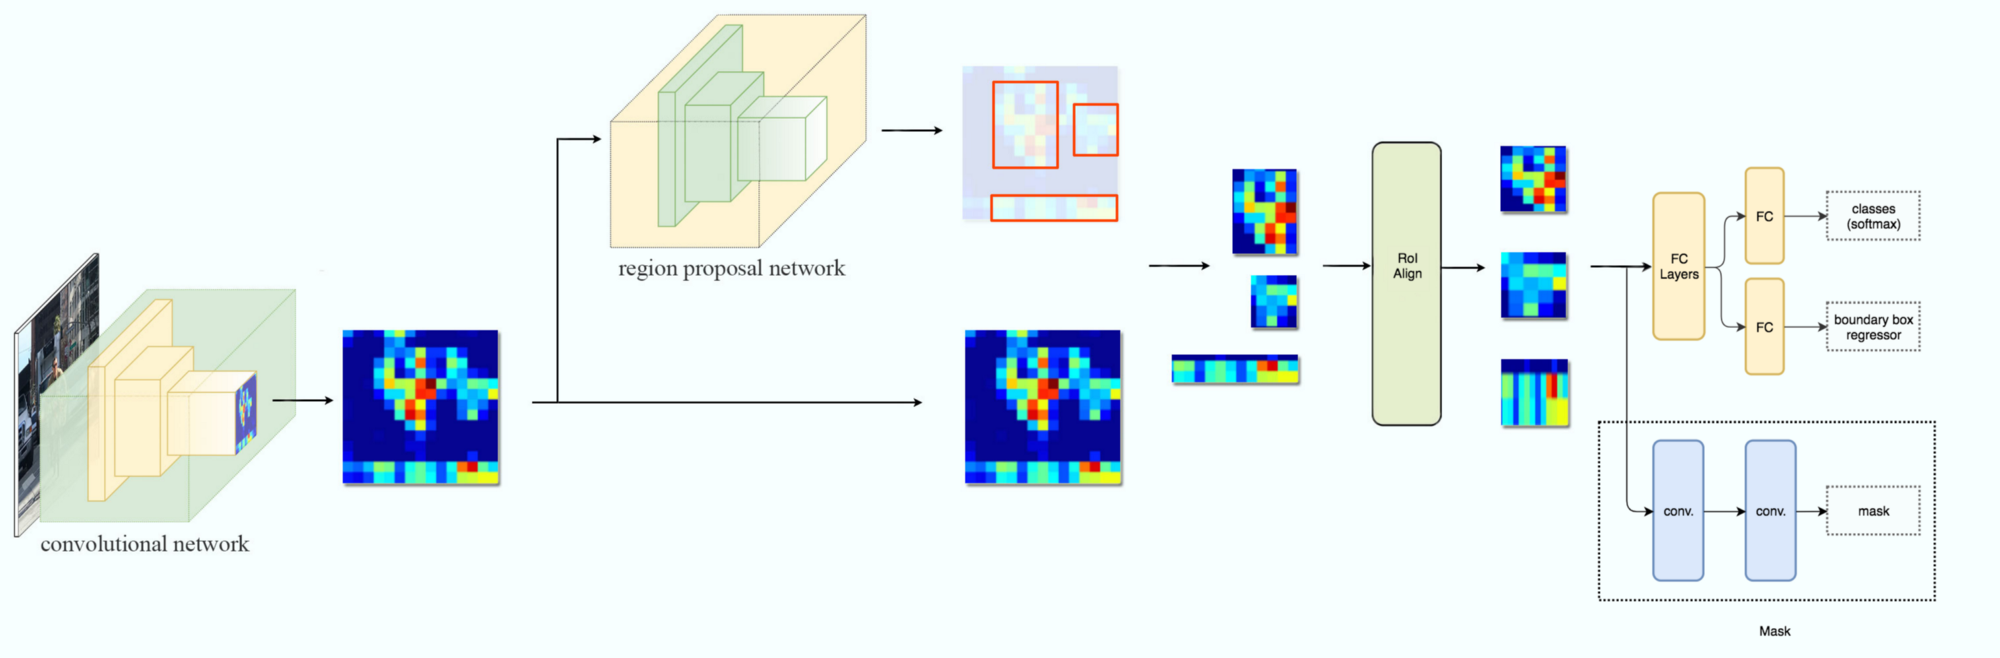
\includegraphics[width=\linewidth]{img/maskrcnn.png}
\caption{Mask R-CNN}
\label{fig_mask-rcnn}
\end{figure}

To understand Mask R-CNN, it works mainly in two stages:

\textbf{Stage1:} The first stage consists of two networks, backbone (ResNet, VGG, Inception, etc..) and region proposal network. These networks run once per image to give a set of region proposals. Region proposals are regions in the feature map which contain the object.

\textbf{Stage2:} In the second stage, the network predicts bounding boxes which is similar to what we have done on Task 1 and object class for each of the proposed region obtained in stage1, in our project this is only one object plant leaf. 
Each proposed region can be of different size whereas fully connected layers in the networks always require fixed size vector to make predictions. Size of these proposed regions is fixed by using either RoI pool (which is very similar to MaxPooling) or RoIAlign method.
The output from RoIAlign layer is then fed into Mask head, which consists of two convolution layers. Mask can be generated for each RoI, thus segmenting leaves pixel-to-pixel.

For our implementation, we convert *\_label.png into mask image and write a adapter for loading dataset.
the original dataset can be splitted into a training set and testing set by our python script.

Because our dataset is not large, and many information like image features can be commonly reused by the different datasets, 
transfer learning \cite{pan2009survey} is used in this project for the training process.
Use the provided pre-trained weight for MS COCO dataset\cite{Lin_2014}.

After data preparation and model construction, the next step is to train the mask-rcnn network.
The training phase is a process to update model parameters and alternate forward and backward propagation.
And the results look pretty good.

\section{Experimental Setup}
\subsection{Task 1}

\subsection{Task2}

\subsection{Task 3}

There are two major problems we've met when finishing this task: 
\begin{itemize}
\item Prepare data for training
\item Evaluating model
\end{itemize}
The reason why the preparation of data becomes hard is because the model we used requires a JSON file to describe features. And the JSON file consists of lots of information, including the names of the files, sizes of files and a few points containing the contours of desired objects. It takes several steps to convert the images to JSON file. 

We first split a label image into several parts \ref{fig_conversion_1}. This allows us to find the contours of the leaves.

\begin{figure}[h!]
    \centering
    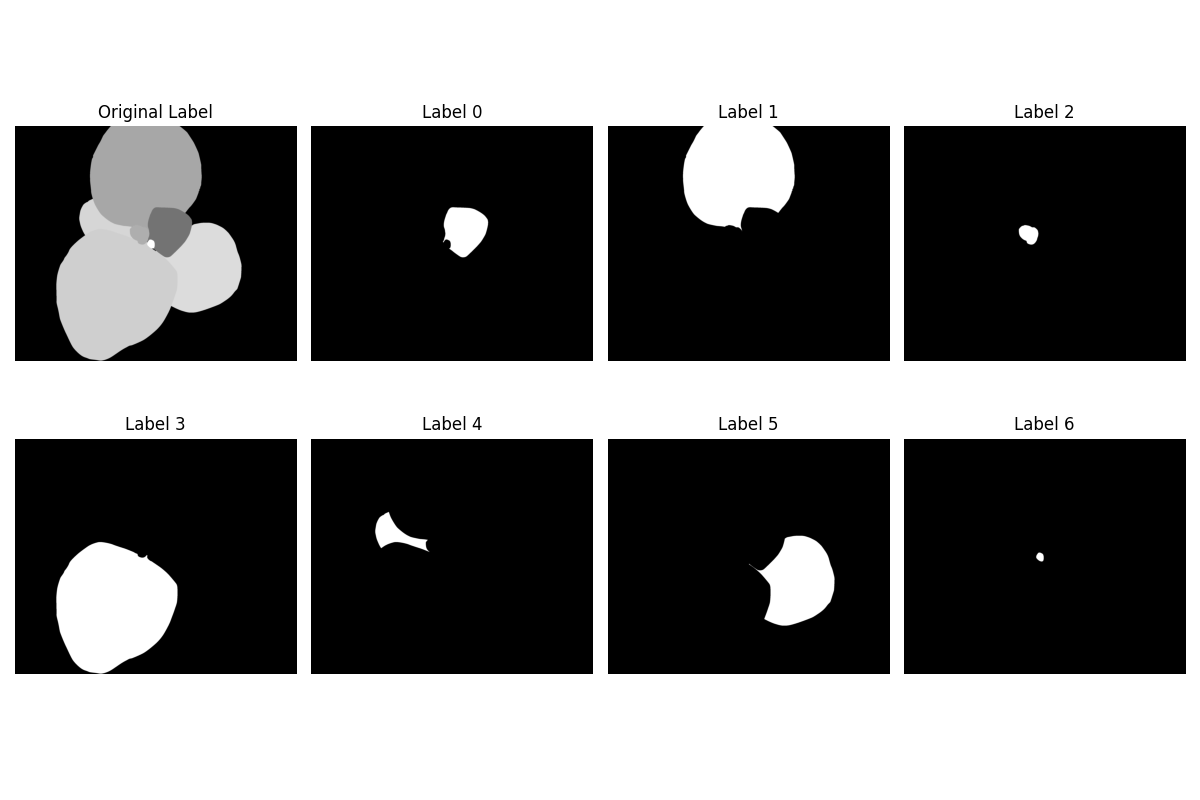
\includegraphics[width=\linewidth]{img/conversion_1.png}
    \caption{Pick single leaves}
    \label{fig_conversion_1}
\end{figure}
To find the contours of the leaves, we can use \verb|cv2.Canny| or \verb|cv2.findContours|. But as the model only need a few points describing the contours, we pick \verb|cv2.findContours| with parameter \verb|method| set to \verb|cv2.CHAIN_APPROX_SIMPLE| and \verb|mode| set to \verb|cv2.RETR_EXTERNAL|. This will generate a series of points denoting a polygon which contains the leaf. 

\begin{figure}[h!]
    \centering
    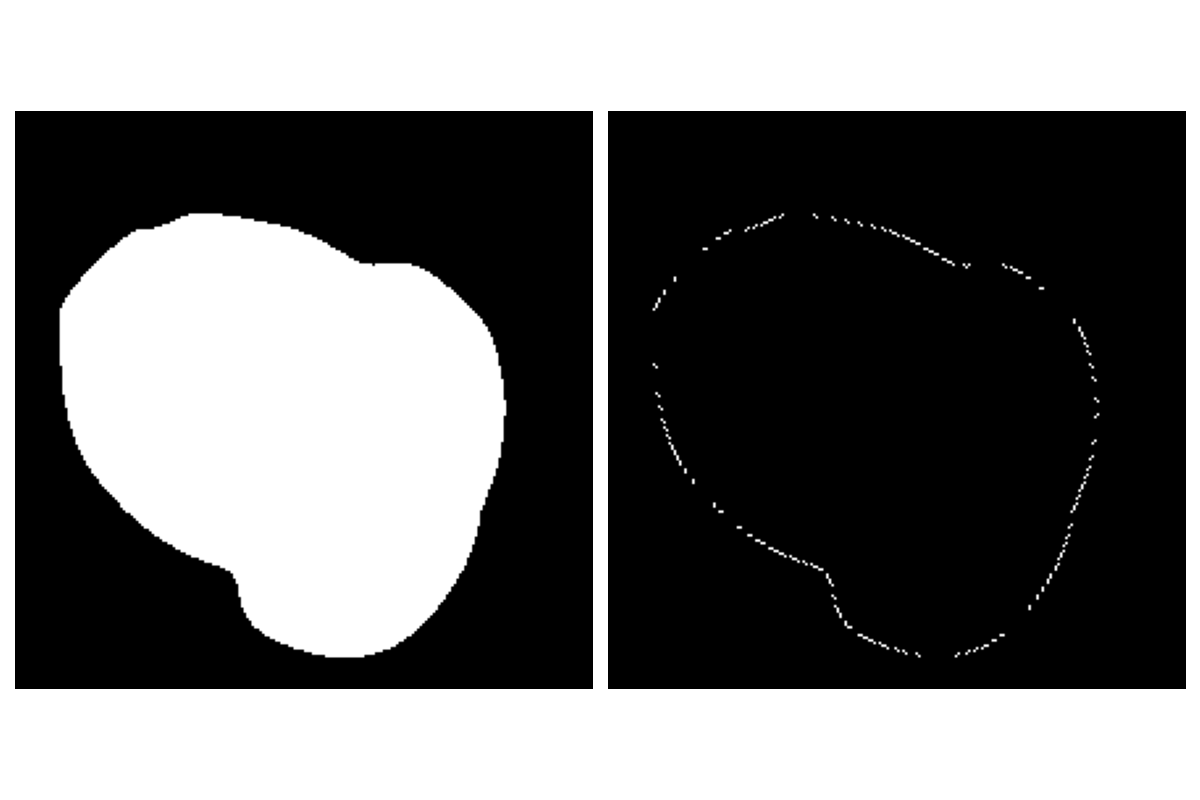
\includegraphics[width=0.75\linewidth]{img/conversion_2_label_2_scaled_up.png}
    \caption{After Processing }
    \label{fig_conversion_2}
\end{figure}
After we got the contours, we can just pick the points in the image and then put them into the JSON file, the preparation of the training data is done.

The second problem is the evaluation. Because we performed the conversion from label images to JSON file, we don't know the relationship of the labels between the output of the model and given labels. Also, the model is not giving us any information about the relation needed for evaluation - which colour maps back to which section of the JSON file. 

Finally, we found the model provided us with the \verb|COCOEvaluator|, which uses the Intersection over Union (\textbf{IoU}) to do the assessment. The Intersection over Union (\textbf{IoU}), also known as \textbf{Jaccard index} is a statistic used for gauging the similarity and diversity of sample sets. The \textbf{Jaccard index} measures similarity between finite sample sets, and is defined as the size of the intersection divided by the size of the union of the sample sets:

\begin{equation}
    J(A,B)=\frac{|A\cap B|}{|A\cup B|}
    \label{eq:IoU}
\end{equation}
You can see this evaluation is pretty close to \textbf{Dice's coefficient}. 

\begin{equation}
	DSC = \frac{2|X \cap Y|}{|X| + |Y|}
	\label{eq:Dice}
\end{equation}
So we looked into the source code of the \verb|COCOEvaluator| and we found a function called \verb|pairwise_iou| which evaluates the result with equation 1. This makes things easier, we can create a \verb|DiceEvaluator| by replacing different function. But we don't want to modify the source code because this makes code harder to maintain. So we created a class called \verb|DiceEvaluator| which inherits the \verb|COCOEvaluator| and a function called \verb|pairwise_dice| which replaces the \verb|pairwise_iou|. 

Though this solution provides us with some flexibility, we are not having fully control over the output. This means that the \verb|DiceEvaluator| always suggests the result is calculated using formula 1. So please notice, in the next section, the output are actually using \textbf{Dice's coefficient} to evaluate the model, not the \textbf{IoU} 


\section{Results and Discussion}

\subsection{Task 1}

\subsection{Task 2}

\subsection{Task 3 Instance Segmentation}

TensorBoard are used to visualize our training process.
Shown on Fig.\ref{fig:loss for training process}.
During the increase of iterations, the model gets stable.
And the total loss drops ideally.

\begin{figure}[h!]
\centering
\begin{subfigure}[h!]{0.24\textwidth}
    \centering
    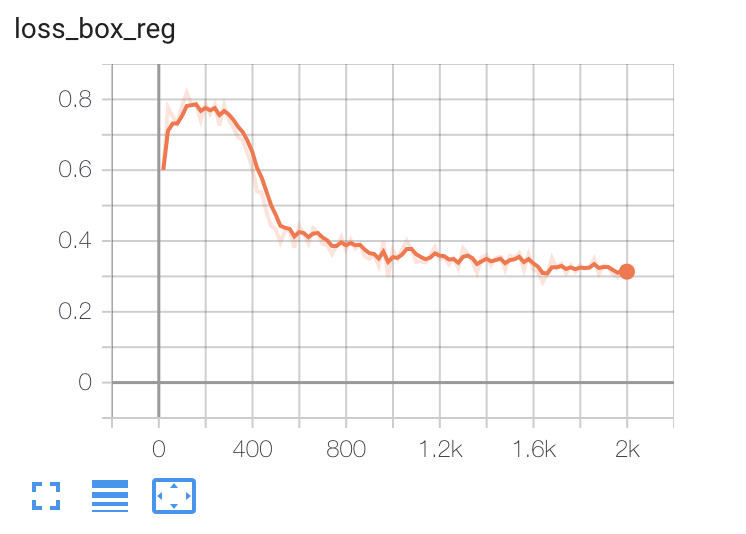
\includegraphics[width=\textwidth]{img/loss_bbox_reg.png}
    \caption{bbox regression loss}
    \label{fig:loss_bbox}
\end{subfigure}
\hfill
\begin{subfigure}[h!]{0.24\textwidth}
    \centering
    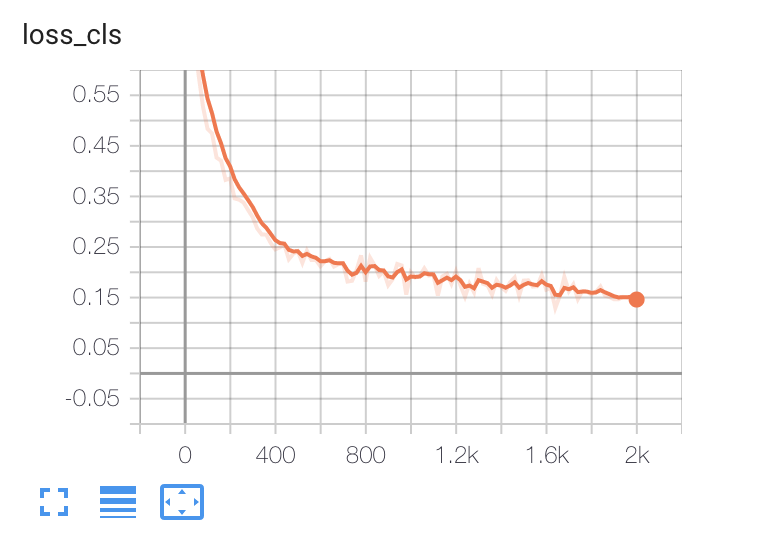
\includegraphics[width=\textwidth]{img/loss_cls.png}
    \caption{classification loss}
    \label{fig:loss_cls}
\end{subfigure}
\hfill
\begin{subfigure}[h!]{0.24\textwidth}
    \centering
    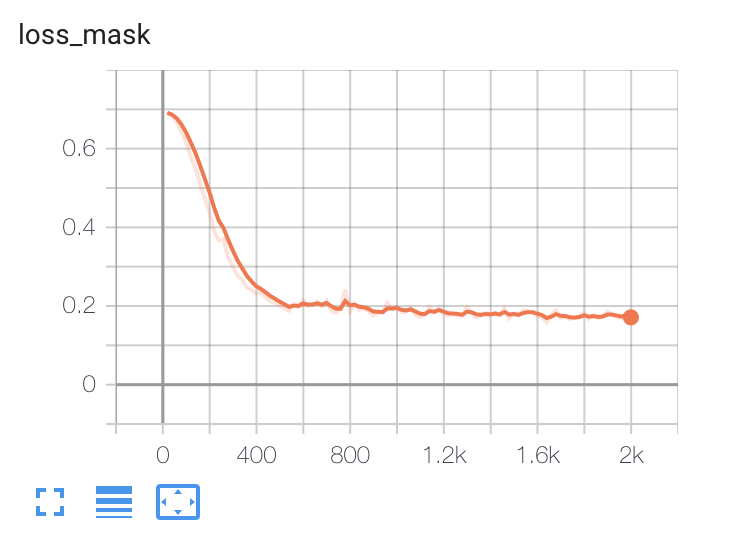
\includegraphics[width=\textwidth]{img/loss_mask.png}
    \caption{mask loss}
    \label{fig:loss_mask}
\end{subfigure}
\hfill
\begin{subfigure}[h!]{0.24\textwidth}
    \centering
    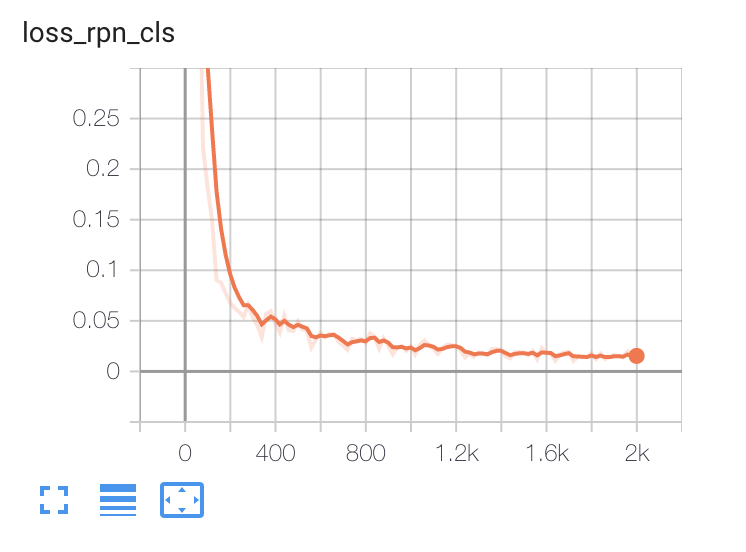
\includegraphics[width=\textwidth]{img/loss_rpn_cls.png}
    \caption{RPN classification loss}
    \label{fig:loss_rpn_cls}
\end{subfigure}
\hfill
\begin{subfigure}[h!]{0.24\textwidth}
    \centering
    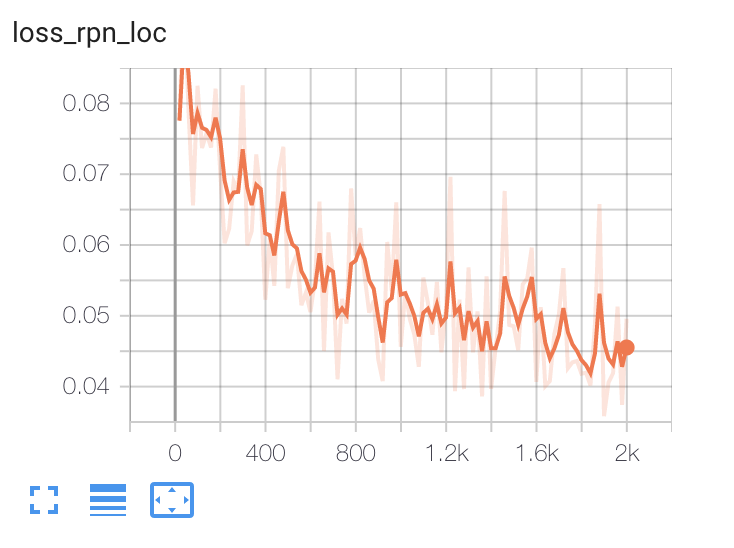
\includegraphics[width=\textwidth]{img/loss_rpn_loc.png}
    \caption{RPN loc loss}
    \label{fig:loss_rpn_loc}
\end{subfigure}
\hfill
\begin{subfigure}[h!]{0.24\textwidth}
    \centering
    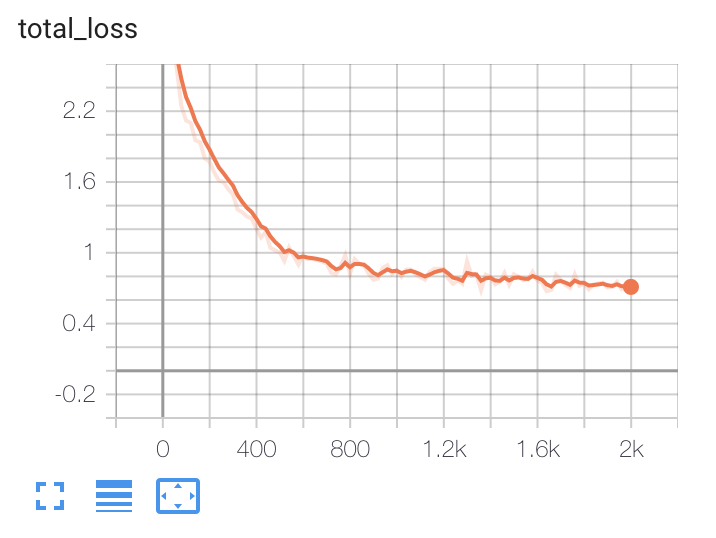
\includegraphics[width=\textwidth]{img/loss_total.png}
    \caption{total loss}
    \label{fig:loss_total}
\end{subfigure}
   \caption{loss for training process}
   \label{fig:loss for training process}
\end{figure}

\begin{figure}[h!]
    \centering
    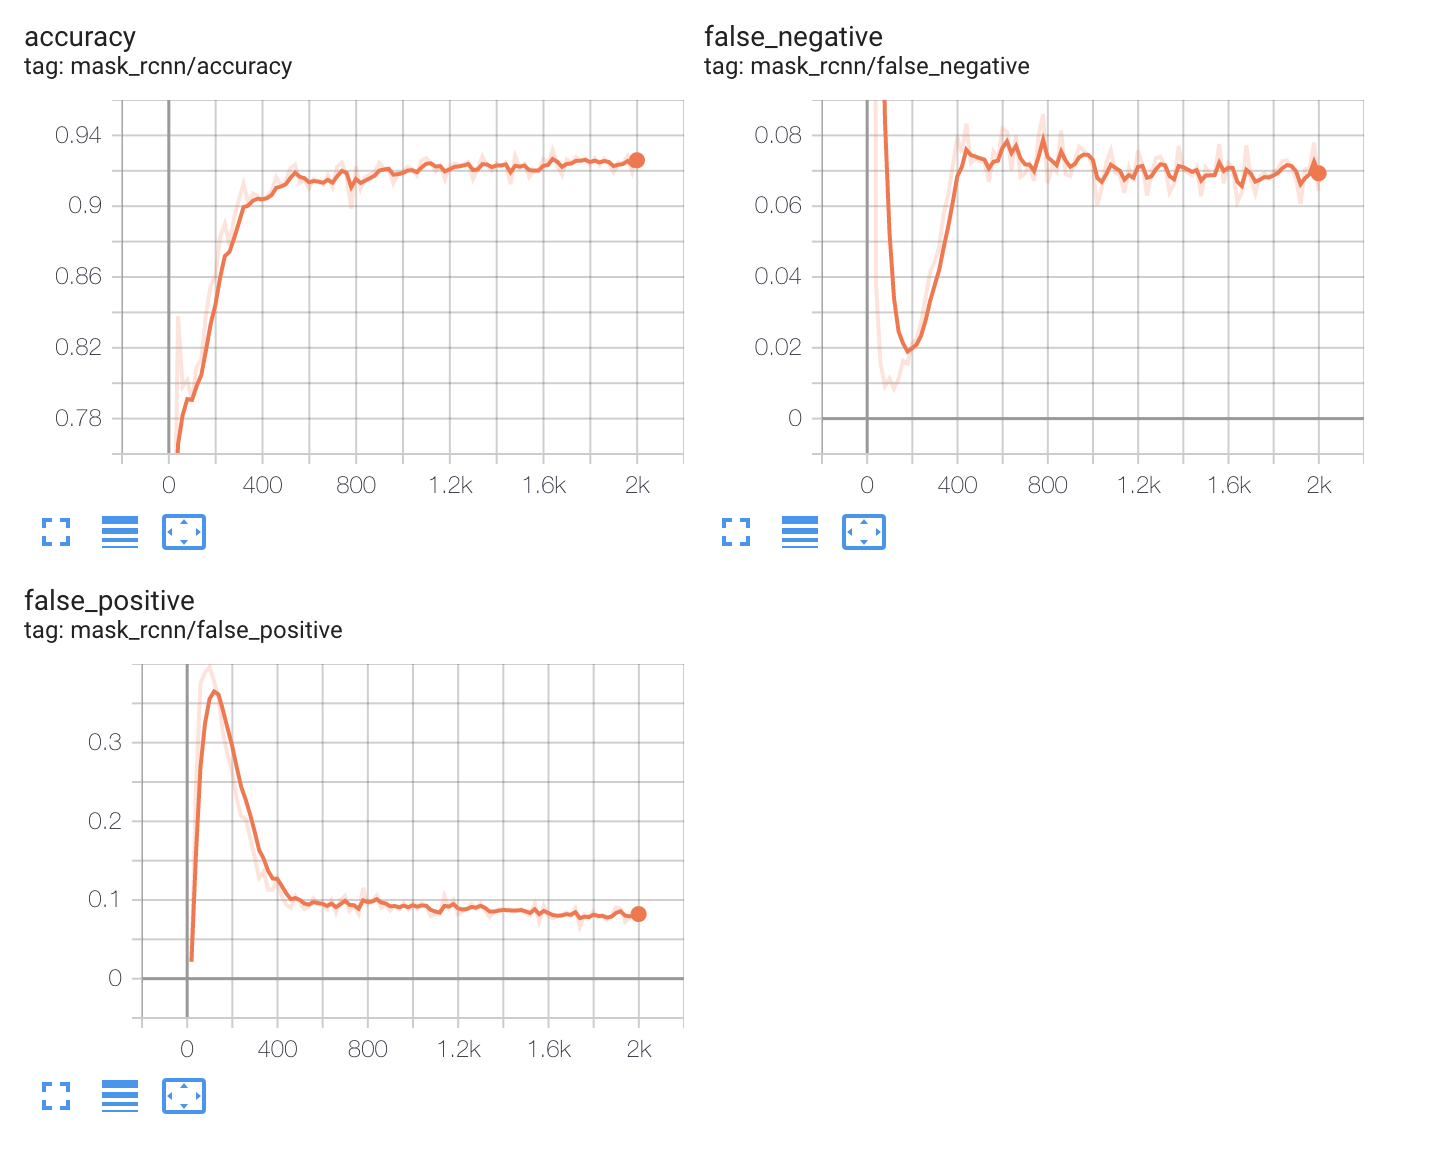
\includegraphics[width=\linewidth]{img/ap_maskrcnn.png}
    \caption{Mask RCNN}
    \label{fig_ap}
\end{figure}

Here are some prediction results. Refer to Fig. \ref{fig:prediction}.
This result of this model shows quite well. 

\begin{figure}[h!]
\centering
\begin{subfigure}[h!]{0.24\textwidth}
    \centering
    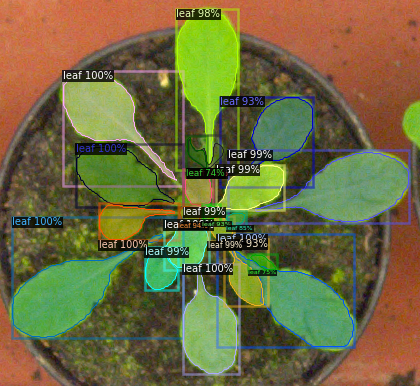
\includegraphics[width=\textwidth]{img/pred1.png}
    % \caption{loss bbox regression}
    % \label{fig:loss_bbox}
\end{subfigure}
\hfill
\begin{subfigure}[h!]{0.24\textwidth}
    \centering
    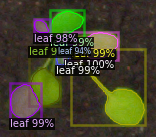
\includegraphics[width=\textwidth]{img/pred2.png}
    % \caption{loss classification}
    % \label{fig:loss_cls}
\end{subfigure}
\hfill
\begin{subfigure}[h!]{0.4\textwidth}
    \centering
    \includegraphics[width=\textwidth]{img/pred3.png}
    % \caption{loss mask}
    % \label{fig:loss_mask}
\end{subfigure}
\caption{Prediction samples}
\label{fig:prediction}
\end{figure}

However, there are still some images not fit well. Refer to Fig.\ref{fig:bad_result}.
Especially these images with low resolution, some leaves do not have a clear boundary,
and some leaves are overlapped with each other. Even human beings cannot distinguish that.

\begin{figure}[h!]
\centering
\begin{subfigure}[h!]{0.24\textwidth}
    \centering
    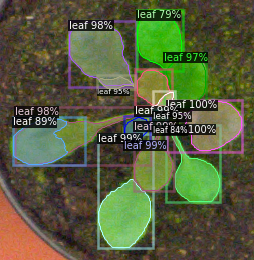
\includegraphics[width=\textwidth]{img/ara2012_plant009.png}
    % \caption{loss bbox regression}
    % \label{fig:loss_bbox}
\end{subfigure}
\hfill
\begin{subfigure}[h!]{0.24\textwidth}
    \centering
    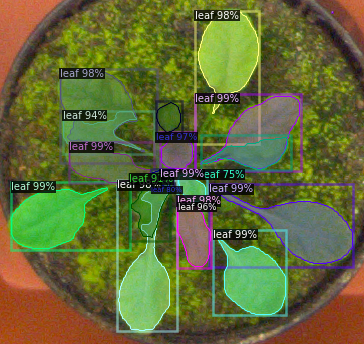
\includegraphics[width=\textwidth]{img/ara2012_plant110.png}
    % \caption{loss classification}
    % \label{fig:loss_cls}
\end{subfigure}
\hfill
\begin{subfigure}[h!]{0.24\textwidth}
    \centering
    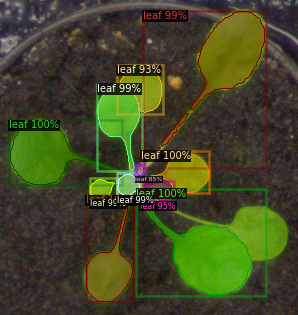
\includegraphics[width=\textwidth]{img/ara2013_plant162.png}
    % \caption{loss mask}
    % \label{fig:loss_mask}
\end{subfigure}
\caption{Some sample images show not so well}
\label{fig:bad_result}
\end{figure}

\begin{figure}[h]
    \centering
    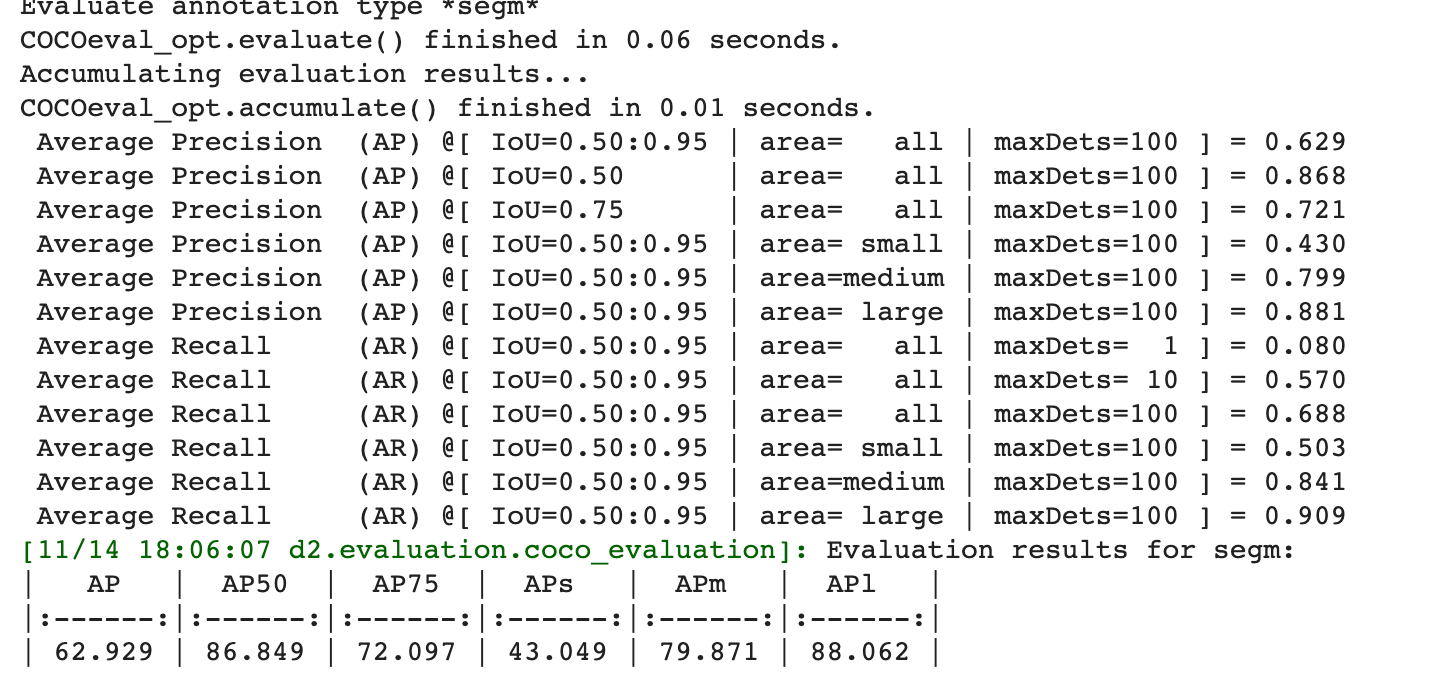
\includegraphics[width=\linewidth]{img/iou_evl.png}
    \caption{Evaluation IoU}
    \label{fig_ap}
\end{figure}


\section{Conclusion}

blabla

\section{Contribution of Group Members}


Task 3:  Yishun Jin, Wei Wang


\bibliographystyle{IEEEtran}
\bibliography{mybib}


\end{document}


